\documentclass[dvipdfmx]{jsarticle}
\usepackage{amsmath,amssymb}
\usepackage[dvipdfmx]{graphicx}
\usepackage{physics}
% table
\usepackage{booktabs}
% unit and No.
\usepackage{siunitx}
% calligraphy
\usepackage{bm}
\usepackage{mathrsfs}
% hyperlink
\usepackage{hyperref}
\usepackage{pxjahyper}
% displaying codes
\usepackage{listings}
% page rotation
\usepackage{lscape}
% subcaption of fig.
\usepackage{subcaption}
% tikz
\usepackage{tikz}
\usepackage{circuitikz}
\usetikzlibrary{intersections,calc,arrows.meta}
\usetikzlibrary{circuits.logic.US}
\usetikzlibrary{positioning, fit}
% eq, fig, table number
\renewcommand{\theequation}{\thesection.\arabic{equation}}
\renewcommand{\thefigure}{\thesection.\arabic{figure}}
\renewcommand{\thetable}{\thesection.\arabic{table}}

\title{宇宙線観察から学ぶ粒子の崩壊とスピン回転
}
\begin{document}
\maketitle

\section{理論}

\subsection{ミュオンの生成}
\label{sec: theory: generation of muon}

ミュオン$\mu^-$は第2世代の荷電レプトンであり、地表に到達する2次宇宙線の大部分を占める。
% 文献裏ドリほしい
電荷は$\pm1$, スピン$1/2$, 質量$\SI[]{105.658 3715(35)}[]{\MeV}$で電子の約200倍あり, 寿命は$\SI{2.1969811(22)}{\micro\second}$である。
% 文献裏ドリほしい
2次宇宙線のミュオンは主に荷電パイオンの崩壊によって生じる。
1次宇宙線の陽子が大気上層で
\begin{align*}
    &p+p\to p+n+\pi^+
    \\
    &p+n\to p+p+\pi^-
    \\
    &p+n\to p+n+\pi^++\pi^-
\end{align*}
の反応を起こしてパイオンが生じ、
\begin{align*}
    &\pi^+\to\mu^++\nu_\mu
    \\
    &\pi^-\to\mu^-+\bar{\nu}_\mu
\end{align*}
と崩壊する。
% 以下全ての反応について、ファインマンダイアグラム描けそうだったら書いて欲しい。必要そうならの話だけど。

ニュートリノのヘリシティは負、反ニュートリノは正であるから、角運動量保存よりパイオン静止系にて$\mu^+$のスピンは運動量と逆、$\mu^-$は同じ向きとなる。
パイオンの崩壊は主に電磁シャワー内部で生じることを考慮すると、実験室系にて地表に降り注ぐ向きの運動量が大きい$\mu^+$はスピンが下向き、$\mu^-$はスピンが上向きになる割合が多くなると考えられる。
% 定量的なことを言いたい
% 図が欲しい気もする


\subsection{ミュオンの崩壊}
\label{sec: theory: decay of muon}

宇宙線ミュオンは地表に降り注ぐ間は固有時間がほとんど進まないが、
% 文献ほしい
資料にトラップされると平均寿命$\SI{2.1969811(22)}{\micro\second}$で崩壊し電子または陽電子を放出する。
\begin{align*}
    &\mu^+\to e^++\nu_e+\bar{\nu}_\mu
    \\
    &\mu^-\to e^-+\bar{\nu}_e+\nu_\mu
\end{align*}
Fermiの黄金則を使えばエネルギーとスピンに依存する(陽)電子の放出方向の分布が計算でき、以下の式で表される。
% 文献ほしい
\begin{equation*}
    \dv{N(v,|b|,t)}{t}
    =
    N_0\frac{\lambda}{2\pi}y^2(3-2y)
    \qty(
        1+\frac{2y-1}{3-2y}P_z\cos\theta
    )
    e^{-\gamma t}\dd{y}\dd{\Omega}
\end{equation*}
積分して、
\begin{equation*}
    N=
    \iint N_0\frac{\lambda}{4\pi}
    A_0(1+aP\cos\theta)e^{-\gamma t}
    \dd{y}\dd{\Omega}
\end{equation*}
を得る。
% 図ほしい。できれば計算で求めたやつ。
すなわち、$\mu^+$はスピンと同じ向きに陽電子を、$\mu^-$はスピンと逆向きに電子を出しやすい。

\ref{sec: theory: generation of muon}を合わせて踏まえると、地表に降り注ぐミュオンのうち運動量の大きいものは上向きに、運動量の小さいものは下向きに(陽)電子を多く放出する。


\subsection{負ミュオンの原子核捕獲}

一部の$\mu^-$は物質中に侵入すると原子核のCoulombポテンシャルにとらわれミュオン原子を形成する。
この$\mu^-$は特性X線やオージェ電子を放出して次第に低準位へ遷移し、やがて原子核へ落ち込む。
原子核にて陽子と弱い相互作用をすることで中性子を放出する。
\begin{equation*}
    \mu^-+p\to n+\nu_\mu
\end{equation*}

(陽)電子だけでなく中性子も検出する装置を使うと、$\mu^-$の減衰比には通常の崩壊に加えてこの原子核捕獲の確率も加わるため、見かけの寿命は$\mu^+$に比べて短くなる。
寿命変化は原子核に依存し、今回使用した試料に含まれる元素では表\ref{table: life of muon}のようになる\cite{Ito Kaji Tabata Yoshiwara}。

% もうちょい桁数ほしい
\begin{table}
    \centering
    \caption{各元素における$\mu^-$の寿命変化}
    \begin{tabular}{lrr}
        \toprule
        元素 & 文献値$[\unit{\micro\second}]$
        \\
        \midrule
        Cu & 0.16
        \\
        Al & 0.86
        \\
        Ca & 0.33
        \\
        C & 2.04
        \\
        O & 0.81
        \\
        \bottomrule
    \end{tabular}
    \label{table: life of muon}
\end{table}

% 元素を混ぜた時の寿命についても書きたい

ミュオンが試料に停止してから崩壊して(陽)電子を出すまでの時間$t$を計測し、$(t,t+\Delta t)$のカウント$N(t)$をヒストグラムで集計すれば、$\mu^-$の寿命変化及び計測のバックグラウンド$BG$を反映して以下の式が成立すると考えられる。
\begin{equation}
    \label{eq: N of t considering different tau and BG}
    N(t)
    =
    N_0^+e^{-t/\tau_+}
    +
    N_0^-e^{-t/\tau_-}
    +
    BG
\end{equation}


\subsection{ミュオンのスピン偏極検出}

\ref{sec: theory: decay of muon}に基づけば、磁場をかけない状態で運動量の比較的大きいミュオンを多くトラップする試料を上下2つの検出器で挟むと上側で(陽)電子をより多く検出する。
しかし上下の検出数の差がスピン偏極によるものなのか検出器の特性によるものなのかを判断することは難しい。
% 実際の実験装置とは別に試料上下に検出器を置いている図が欲しい。概念的なものなのでTはいらない。

磁気回転比$\gamma$のミュオンスピンに磁場$\bm{B}$がかかると、
\begin{equation}
    \label{eq: Larmor precession}
    \bm{\omega}=\gamma\bm{B}
\end{equation}
の角速度で歳差運動を行う(Larmor歳差運動)。
これを使うことで上記の問題が解決できる。

上下の検出器でのカウントをそれぞれ$N_U, N_D$とする。
\ref{sec: theory: decay of muon}で述べた$\mu^-$の原子核捕獲も考慮すると、以下の式が成り立つと考えられる。
\begin{equation}
    \label{eq: N under Larmor}
    \begin{split}
        N_U
        &=
        N_{U0}^+(1+AP^+\cos\omega t)e^{-t/\tau_+}
        +
        N_{U0}^-(1+AP^-\cos\omega t)e^{-t/\tau_-}
        +
        BG_D
        \\
        N_D
        &=
        N_{D0}^+(1-AP^+\cos\omega t)e^{-t/\tau_+}
        +
        N_{D0}^-(1-AP^-\cos\omega t)e^{-t/\tau_-}
        +
        BG_D
    \end{split}
\end{equation}
ここで$\tau_-$は原子核捕獲のため一般に小さく、$\mu^-$は試料に侵入すると周囲の電子との間で相互作用してスピン偏極が破れる。
% 文献ほしい
このため$t\gg\tau_-$にて\eqref{eq: N under Larmor}各式の第2項は無視できる。
$N_U'=N_U-BG_U, N_D'=N_D-BG_D$及び実数$\alpha$を使って、
\begin{equation}
    \label{eq: asymmetry}
    \mathscr{A}
    =
    \frac{\alpha N_U'-N_D'}{\alpha N_U'+N_D'}
    =
    \frac{(\alpha N_{U0}^+-N_{D0}^+)+(\alpha N_{U0}^++N_{D0}^+)AP^+\cos\omega t}{(\alpha N_{U0}^++N_{D0}^+)+(\alpha N_{U0}^+-N_{D0}^+)AP^+\cos\omega t}
\end{equation}
と表される非対称度は、$\alpha N_{U0}^+-N_{D0}^+=0$なる$\alpha$にて角振動数$\omega$の三角関数となる。


\section{実験・解析方法}
\subsection{寿命測定}

\begin{figure}
    \centering
    \begin{tabular}[]{ccc}
        \begin{minipage}[t]{0.3\hsize}
            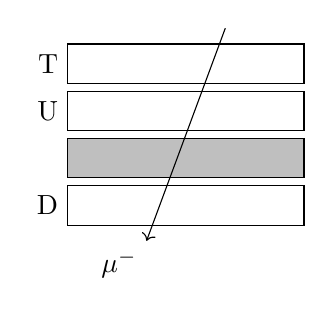
\begin{tikzpicture}
    \draw(0,0)rectangle(3,0.5);
    \fill[lightgray](0,0.6)--(0,1.1)--(3,1.1)--(3,0.6)--cycle;
    \draw(0,0.6)rectangle(3,1.1);
    \draw(0,1.2)rectangle(3,1.7);
    \draw(0,1.8)rectangle(3,2.3);
    \draw[->] (2,2.5)--(1,-0.2) node [below left]{$\mu^{-}$};
    \node [left] at (0,2.05){T};
    \node [left] at (0,1.45){U};
    \node [left] at (0,0.25){D};
\end{tikzpicture}

            \subcaption{試料を通過する場合}
        \end{minipage}
        &
        \begin{minipage}[t]{0.3\hsize}
            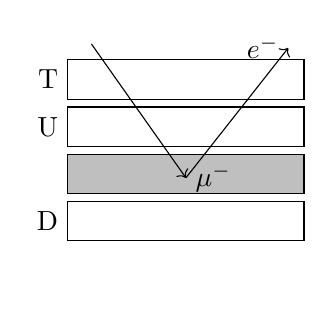
\begin{tikzpicture}
    \draw(0,0)rectangle(3,0.5);
    \fill[lightgray](0,0.6)--(0,1.1)--(3,1.1)--(3,0.6)--cycle;
    \draw(0,0.6)rectangle(3,1.1);
    \draw(0,1.2)rectangle(3,1.7);
    \draw(0,1.8)rectangle(3,2.3);
    \node [left] at (0,2.05){T};
    \node [left] at (0,1.45){U};
    \node [left] at (0,0.25){D};
    \node [below] at (1,-0.2){\textcolor{white}{$\nu_\mu$}}; %高さ調整
    \draw[->] (0.3,2.5)--(1.5,0.8) node [right]{$\mu^{-}$};
    \draw[->] (1.5,0.8)--(2.8,2.45) node [left]{$e^{-}$};
\end{tikzpicture}

            \subcaption{崩壊してUに電子を飛ばす場合}
        \end{minipage}
        &
        \begin{minipage}[t]{0.3\hsize}
            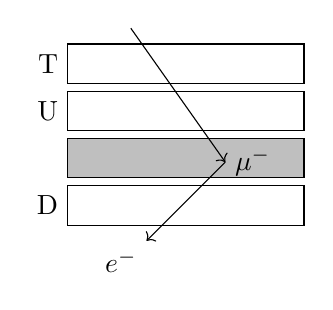
\begin{tikzpicture}
    \draw(0,0)rectangle(3,0.5);
    \fill[lightgray](0,0.6)--(0,1.1)--(3,1.1)--(3,0.6)--cycle;
    \draw(0,0.6)rectangle(3,1.1);
    \draw(0,1.2)rectangle(3,1.7);
    \draw(0,1.8)rectangle(3,2.3);
    \draw[->] (0.8,2.5)--(2,0.8) node [right]{$\mu^{-}$};
    \draw[->] (2,0.8)--(1,-0.2) node [below left]{$e^{-}$};
    \node [left] at (0,2.05){T};
    \node [left] at (0,1.45){U};
    \node [left] at (0,0.25){D};
\end{tikzpicture}

            \subcaption{崩壊してDに電子を飛ばす場合}
        \end{minipage}
    \end{tabular}
    \caption{PSc+PMTの配置と粒子の飛程}
    \label{img: PSc, PMT position and muon path}
\end{figure}

\begin{figure}
    \centering
    \begin{circuitikz}
    \draw
    (1,0)
    % BTUnotD
    node[ieeestd and port, number inputs=3, anchor=in 1] (BTUnotD) {}
    % T
    (BTUnotD.in 1) -- ++(-1,0)
    node[anchor=east] {T}
    % GG
    (BTUnotD.out) to[short] ++(0.5,0)
    node[twoportshape, anchor=west, t=GG](GG){} ++(1,0)
    % to D stop
    -- ++(0.5,0)
    to [short, *-] ++(0,-1.5)
    -- ++(1,0)
    node[ieeestd and port, anchor=in 1] (Dstop){}
    (Dstop.out) node[anchor=west]{D stop};
    % not D
    \node at (BTUnotD.bin 3) [ocirc, left]{};
    % GG to U stop
    \draw
    (GG.east)
    to [short] ++(1.5,0)
    node[ieeestd and port, anchor=in 1](Ustop){}
    (Ustop.out) node[anchor=west]{U stop};
    \draw
    (BTUnotD.out) to[short, *-] ++(0,1)
    to[short] ++(5.2,0)
    node[anchor=west](start){start};
    \draw
    (BTUnotD.in 2) to[short] ++(-1,0)
    node[anchor=east](U){U}
    (BTUnotD.in 3) to[short] ++(-1,0)
    node[anchor=east](D){D}
    (0.5,-0.38) to [short, *-] ++(0,-1)
    -- ++(1,0)
    -| (Ustop.in 2)
    (0.7, -0.75) to [short, *-] ++(0,-1.4)
    |- (Dstop.in 2)
    ;
\end{circuitikz}

    \caption{回路の概要}
    \label{img: circuit easy}
\end{figure}

\subsection{スピン偏極測定}


\section{結果・考察}
\subsection{ミュオンの寿命}

\subsection{スピン偏極}


\pagebreak



\appendix
\setcounter{section}{0}
\setcounter{equation}{1}
\setcounter{figure}{1}
\setcounter{table}{1}
\renewcommand{\theequation}{\Alph{section}.\arabic{equation} }
\renewcommand{\thefigure}{\Alph{section}.\arabic{equation} }
\renewcommand{\thetable}{\Alph{section}.\arabic{equation} }

\section{論理回路}
実験で実際に用いたNIMモジュールの回路を図\ref{img: full circuit}に掲げる。
主にCu, Alからの信号の入力部(Cu, Al)、大理石からの入力部($\mathrm{CaCO_3}$)、制御部(GATES)、出力部(OUTPUTS)に大別できる。

入力はTUD各層それぞれ3組のPSc+PMTから引いている。
それぞれT1, T2, T3, U1, ...と番号を振っている。
Cu, AlのTに描いたようなor接続をCu, AlのU以下全ての入力端子でとっているが、簡単のためCu, AlのT以外は省略した。
なお、このor接続以前でdelayを置いているのはCu, AlのTのみである。

制御部GATESはCu, Alと大理石の信号が干渉しないようにスイッチの役割を果たす。
具体的には、Cu, Al側のGGが起動している間は大理石の信号が入ってもstopと判定しない。
逆もまた然りである。

DAQ-PCでは短時間に複数のstart信号を受けたとき最初の信号のみを使用し、それ以降の信号は無視する。

\begin{landscape}
    \begin{figure}
        \centering
        % displaying the circuit without rotation
\begin{circuitikz}
    % B
    \draw
        (1,0)
        % TUnotD
        node[ieeestd and port, number inputs=3, anchor=in 1] (BTUnotD) {}
        % T
        (BTUnotD.in 1) to[short] ++(-1,0)
        node[anchor=east](BT){$\mathrm{CaCO_3}$ T}
        % gateBlocal
        (BTUnotD.out) to[short] ++(0.5,0)
        node[twoportshape, anchor=west, t=GG] (gateBlocal){} ++(1,0)
        % gate delay
        to [short] ++(0.5,0)
        node[align=left, anchor=west](gateBdelay){\small delay\\$\SI{31}{\nano\second}$} ++(1,0)
        % to D stop
        to [short] ++(0.5,0)
        to [short, *-] ++(0,-1.5)
        to [short] ++(0.55,0)
        node[ieeestd and port, anchor=in 1] (BDstoplocal){}
        % (BDstoplocal.out) node[anchor=west]{D stop}
        ;
        % not D
        \node
        at (BTUnotD.bin 3) [ocirc, left]{}
        ;
        % gateBdelay to U stop
        \draw
        (gateBdelay.east)
        to [short] ++(1,0)
        node[ieeestd and port, anchor=in 1](BUstoplocal){} ++(1,0)
        % (BUstoplocal.out) node[anchor=west]{U stop}
        ;
        % start
        \draw
        (BTUnotD.out) to[short, *-] ++(0,1)
        to[short] ++(3.5,0)
        node[anchor=west](Bstart){}
        ;
        \draw
        (BTUnotD.in 2) to[short] ++(-1,0)
        node[anchor=east](U){$\mathrm{CaCO_3}$ U}
        (BTUnotD.in 3) to[short] ++(-1,0)
        node[anchor=east](D){$\mathrm{CaCO_3}$ D}
        (0.5,-0.38) to [short, *-] ++(0,-1)
        -- ++(2,0)
        node[align=left, anchor=west]{\small delay\\ $\SI{2}{\nano\second}$} ++(1,0)
        -| (BUstoplocal.in 2)
        (0.7, -0.75) to [short, *-] ++(0,-1.4)
        |- (BDstoplocal.in 2)
        % node [anchor=north](Ddelay){delay}
        % (Ddelay.east) -- (BDstoplocal.in 2)
        % U stop
        (15,-0.3) node[ieeestd and port, anchor=center, number inputs=3](BUstop){}
        (BUstop.out) node[anchor=west]{$\mathrm{CaCO_3}$ U stop}
        % D stop
        (15,-1.8) node[ieeestd and port, anchor=center, number inputs=3](BDstop){}
        (BDstop.out) node[anchor=west](BDstopLabel){$\mathrm{CaCO_3}$ D stop}
        (BUstoplocal.out) -- (BUstop.in 3)
        (BDstoplocal.out) -- (BDstop.in 3)
        ;
        % box
        \node[rectangle,draw,dashed,fit=(BT) (BDstoplocal) (BDstoplocal)](CaCO3){};
        \node[anchor=north, align=center] at (CaCO3.south){$\mathrm{CaCO_3\:INPUTS}$};
    % A
    \draw
        % T
        (2,6)
        node[ieeestd or port, number inputs=3, anchor=in 1] (ATor) {}
        % T1E
        (0,7) node[anchor=east](T1E){Cu, Al T1}
        -- ++(1.2,0)
        node[align=left, anchor=west](T1Edelay){\small delay\\ $\SI{22}{\nano\second}$} (1,0)
        (T1Edelay.south) |- (ATor.in 1)
        % T2E
        (0,5.62)
        node[anchor=east]{Cu, Al T2}
        -- ++(0.5,0)
        node[align=left, anchor=west](T2Edelay){\small delay\\ $\SI{14}{\nano\second}$} (1,0)
        (T2Edelay.east) -- (ATor.in 2)
        % T3E
        (0,4.5)
        node[anchor=east]{Cu, Al T3}
        -- ++(1.2,0)
        node[align=left, anchor=west](T3Edelay){\small delay\\ $\SI{30}{\nano\second}$}
        (T3Edelay.north) |- (ATor.in 3)
        ;
        \draw
        % TUnotD
        (4.5,3.625)
        node[ieeestd and port, number inputs=3, anchor=in 1](ATUnotD){}
        (ATor.out) |- (ATUnotD.in 1)
        % U
        (ATUnotD.in 2)
        to[short] (0,3.25)
        node[anchor=east]{Cu, Al U}
        % D
        (ATUnotD.in 3)
        to[short] (0,2.9)
        node[anchor=east](AD){Cu, Al D}
        ;
        % not D
        \node at (ATUnotD.bin 3) [ocirc, left]{};
        % AU stop
        \draw
        (15,8) node[ieeestd and port, anchor=center, number inputs=3](AUstop){}
        ;
        \draw
        % U to Ustop
        (3,3.25)
        to [short, *-] ++(0,1.5)
        -| ++(2,3.6)
        -- ++(1,0)
        node[anchor=west, align=left]{\small delay\\ $\SI{30}{\nano\second}$} ++(1,0)
        % to [short] ++(1,0)
        -- (AUstop.in 1)
        % AD stop
        (15,6.5) node[ieeestd and port, anchor=center, number inputs=3](ADstop){}
        ;
        % D to Dstop
        \draw
        (3.5,2.9)
        to [short, *-] ++(0,1.2)
        -| ++(2,3.2)
        to [short] ++(1,0)
        -| (ADstop.in 1)
        (AUstop.out) node[anchor=west](AUstopLabel){Cu, Al U stop}
        (ADstop.out) node[anchor=west]{Cu, Al D stop}
        ;
        % box
        \node[rectangle,draw,dashed,fit=(T1E) (AD) (ATUnotD) (T1Edelay)](CuAl){};
        \node[anchor=north, align=center] at (CuAl.south){Cu, Al INPUTS};
    % gate
    \draw
        % and9
        (10,2.97)
        node[ieeestd and port, anchor=center](and9){}
        % and10
        (10,5)
        node[ieeestd and port, anchor=center](and10){}
        % ATUnotD to 9
        (ATUnotD.out) |- (and9.in 1)
        % gateA
        (8.2,6.5) node[twoportshape, anchor=center, t=GG](gateA){}
        % gateB
        (8.2,1) node[twoportshape, anchor=center, t=GG](gateB){}
        (Bstart.west) |- (and10.in 2)
        % start trigger
        (15,4)
        node[ieeestd or port, anchor=center](STARTor){}
        (STARTor.out) node[anchor=west]{start}
        % 9 and 10 to start or
        (and9.out) |- (STARTor.in 2)
        (and10.out) |- (STARTor.in 1)
        % 9 to gate A
        (and9.out) to [short, *-] ++(0,-1)
        to [short] ++(-4,0)
        |- (gateA.west)
        % 10 to gate B
        (and10.out) to [short, *-] ++(0,0.9)
        to [short] ++(-3.7,0)
        |- (gateB.west)
        ;
        \draw
        % gate B to BU stop
        (gateB.east) to[short, -*] (13,1)
        |- (BDstop.in 2)
        % gate B to BD stop
        (13,-0.3) to[short, *-] (BUstop.in 2)
        % gate B to A stop
        (gateB.east) -- (13,1)
        |- (AUstop.in 3)
        (13,6.13) to[short, *-] (ADstop.in 3)
        ;
        \node
        at (AUstop.bin 3) [ocirc, left]{}
        ;
        \node
        at (ADstop.bin 3) [ocirc, left]{}
        ;
        % gate B to 9
        \draw
        (gateB.east) to[short] ++(0.2,0)
        to [short, *-] ++(0,0.2)
        |- (and9.in 2)
        ;
        \node
        at (and9.bin 2) [ocirc, left]{}
        ;
        % gate A to 10
        \draw
        (gateA.east) to[short] ++(0.2,0)
        to [short, *-] ++(0,-0.2)
        |- (and10.in 1)
        ;
        \node
        at (and10.bin 1) [ocirc, left]{}
        ;
        \draw
        % gate A to A stop
        (12,6.5) to[short, *-] ++(0,1.5)
        -- (AUstop.in 2)
        (12,6.5) -- (ADstop.in 2)
        % gate A to B stop
        (gateA.east) to[short] (12,6.5)
        |- (BDstop.in 1)
        ;
        \node
        at (BDstop.bin 1) [ocirc, left]{}
        ;
        \draw
        (12,0.06) to[short, *-] (BUstop.in 1)
        ;
        \node
        at (BUstop.bin 1) [ocirc, left]{}
        ;
        % box
        \node[rectangle,draw,dashed,fit=(gateA) (gateB) (and9) (and10)](gates){};
        \node[anchor=north east, align=left] at (gates.south east){GATES};
    % outputs box
    \node[rectangle,draw,dashed,fit=(AUstop)(BDstop)(AUstopLabel)(BDstopLabel)](outputs){};
    \node[anchor=north, align=center]at(outputs.south){OUTPUTS};
\end{circuitikz}

        \caption{実験で用いた論理回路}
        \label{img: full circuit}
    \end{figure}
\end{landscape}

\begin{thebibliography}{10}
    \bibitem{Ito Kaji Tabata Yoshiwara} 伊藤泰男,鍛冶東海,田畑米穂,吉原賢二,「素粒子の化学」学会出版センター(1985)
\end{thebibliography}
\end{document}
